% =============================================================
%  Reusable-Vehicle Flight Clearance — Payload2026
%  Stage 0->3 Bayesian SHM stack, rocket-context demo  (2026-06)
% =============================================================
\documentclass[aspectratio=169, 10pt]{beamer}
\usetheme[progressbar=frametitle, block=fill]{metropolis}
\usepackage[T1]{fontenc}
\usepackage{newtxtext, newtxmath}
\usepackage{microtype}
\usepackage{booktabs}
\usepackage{colortbl}
\usepackage{graphicx}
\usepackage{amsmath, amssymb}
\usepackage{tikz}
\usetikzlibrary{arrows.meta, positioning}

\definecolor{luhblue}{RGB}{0,80,155}
\definecolor{okgreen}{RGB}{27,94,32}
\definecolor{alertred}{RGB}{198,40,40}
\setbeamercolor{frametitle}{bg=luhblue, fg=white}
\setbeamercolor{progress bar}{fg=luhblue}
\setbeamercolor{alerted text}{fg=alertred}
\setbeamercolor{example text}{fg=okgreen}
\metroset{progressbar=frametitle, block=fill}
\newcommand{\best}[1]{\textbf{\textcolor{luhblue}{#1}}}

\setbeamerfont{page number in head/foot}{size=\scriptsize}
\setbeamertemplate{footline}{%
  \hbox{\begin{beamercolorbox}[wd=\paperwidth, ht=2.6ex, dp=1.2ex, leftskip=2ex,
    rightskip=2ex]{}%
    \scriptsize Reusable-vehicle flight clearance \hfill
    \insertframenumber\,/\,\inserttotalframenumber%
  \end{beamercolorbox}}}

% Logos top-right, graceful if files absent. Drop official files in slides/:
%   keio-logo.{pdf,png}  luh-logo.{pdf,png}  jaxa-logo.{pdf,png}
\newcommand{\maybelogo}[1]{%
  \IfFileExists{#1.pdf}{\includegraphics[height=6mm]{#1}\hspace{2mm}}{%
    \IfFileExists{#1.png}{\includegraphics[height=6mm]{#1}\hspace{2mm}}{}}}
\addtobeamertemplate{frametitle}{}{%
  \begin{tikzpicture}[remember picture, overlay]
    \node[anchor=north east, xshift=-3mm, yshift=-1.2mm] at (current page.north east){%
      \maybelogo{keio-logo}\maybelogo{luh-logo}\maybelogo{jaxa-logo}};
  \end{tikzpicture}}

\title{Reusable-Vehicle Flight Clearance}
\subtitle{From guided-wave SHM to a go/no-go decision with uncertainty}
\author{Keisuke Nishioka}
\institute{Payload2026 \quad$\cdot$\quad LUH / Keio}
\date{June 2026}

\begin{document}
\maketitle

% ─────────────────────────────────────────────
\begin{frame}{The reusable-vehicle question}
\begin{columns}[T]
\column{0.56\textwidth}
H3 fairing SHM so far: \best{detect \& localise} debonding from guided waves
(SAGE F1 0.79, LGSTA 0.86).\\[2mm]
For a \alert{reusable} stage the question becomes:
\begin{itemize}
  \item is this fairing/stage OK to fly \emph{again}?
  \item how many flights remain, with what confidence?
\end{itemize}
\column{0.42\textwidth}
\begin{block}{New layer}
Turn the SHM posterior into a calibrated
\textbf{flight-clearance decision} via phase-field crack prognosis.
\end{block}
\end{columns}
\end{frame}

% ─────────────────────────────────────────────
\begin{frame}{Pipeline: measurement to decision}
\centering
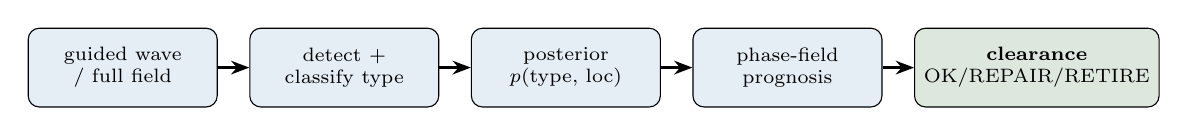
\begin{tikzpicture}[
  box/.style={draw, rounded corners, fill=luhblue!10, minimum width=2.4cm,
              minimum height=10mm, align=center, font=\scriptsize},
  arr/.style={-{Stealth}, thick}]
\node[box] (m) {guided wave\\ / full field};
\node[box, right=4mm of m] (d) {detect +\\ classify type};
\node[box, right=4mm of d] (c) {posterior\\ $p(\text{type, loc})$};
\node[box, right=4mm of c] (p) {phase-field\\ prognosis};
\node[box, fill=okgreen!15, right=4mm of p] (g) {\textbf{clearance}\\ OK/REPAIR/RETIRE};
\draw[arr] (m)--(d); \draw[arr] (d)--(c); \draw[arr] (c)--(p); \draw[arr] (p)--(g);
\end{tikzpicture}\\[3mm]
\begin{itemize}\footnotesize
  \item detect+classify: GNN on 9 sensor nodes $\times$ 24 features
        (SAGE F1 0.79, LGSTA 0.86); guided waves 16.5--300\,kHz
  \item type/location posterior: long-term tags (13 damage states) +
        5-class FEM localisation ($z\times\theta$ quadrants),
        \emph{temperature-scaled, ECE-reported}
  \item prognosis: anisotropic AT2 + interface bands + Carrara-2020 fatigue
        $\Rightarrow$ $P(\text{survive }n)$, $\mathbb{E}[\text{flights}]$
  \item caveat: long-term tags carry a temporal confound
        (months differ in temperature \& aging) --- reported, not hidden
\end{itemize}
\end{frame}

% ─────────────────────────────────────────────
\begin{frame}{Flight clearance --- demo (real posterior, fatigue on/off)}
\begin{columns}[T]
\column{0.50\textwidth}
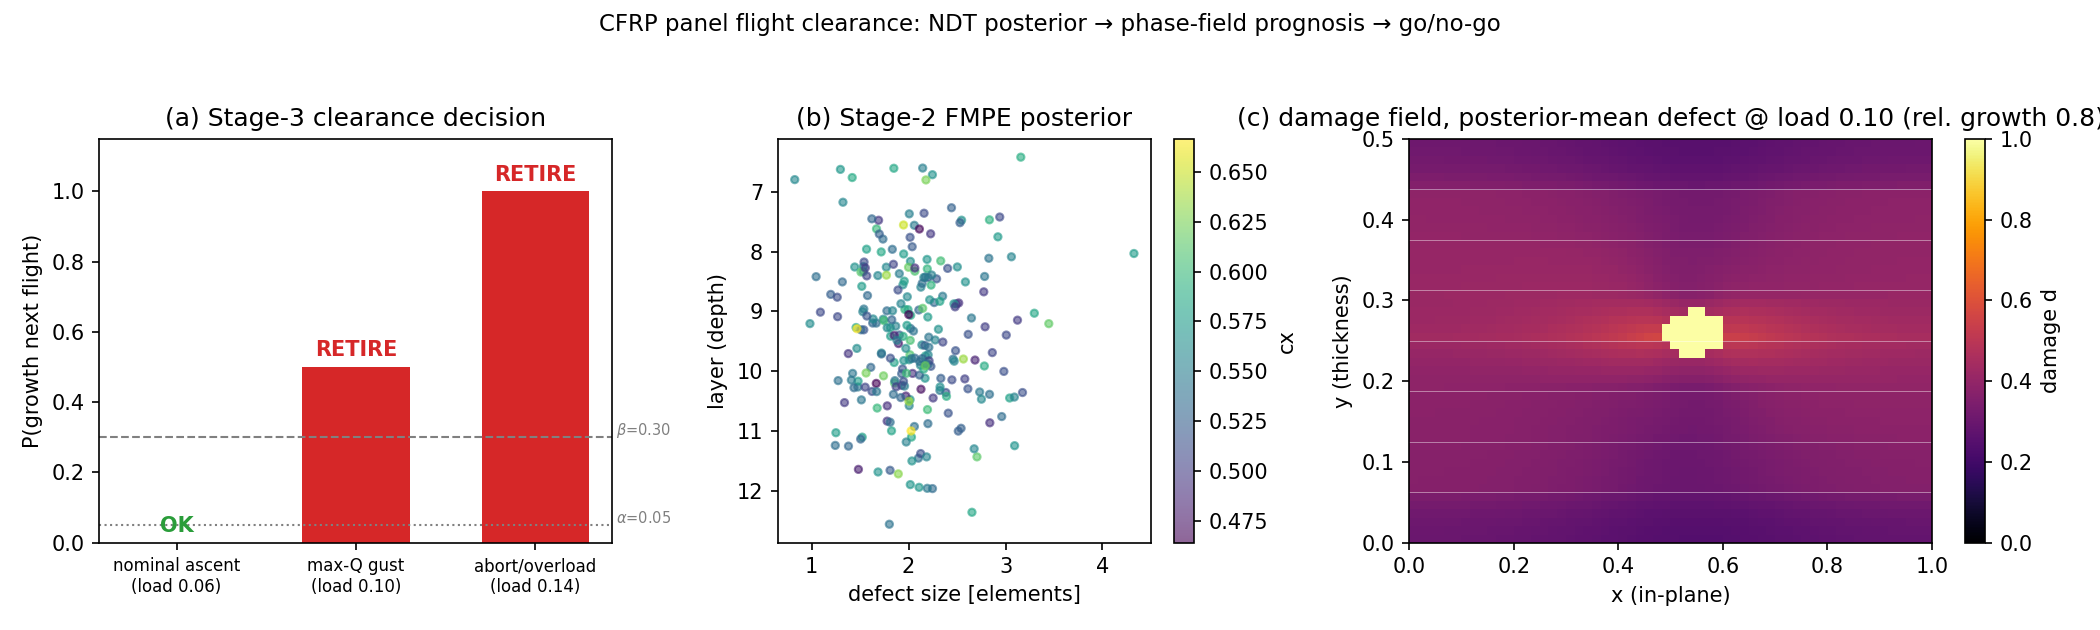
\includegraphics[width=\textwidth]{../results/flight_clearance_demo.png}
\column{0.48\textwidth}
\scriptsize
\begin{tabular}{lccc}
\toprule
load & fatigue & $\mathbb{E}[\text{flights}]$ & decision \\
\midrule
nominal & ON  & \textbf{19.9} & \textcolor{okgreen}{\textbf{OK}} \\
nominal & off & 11.0 & \textcolor{okgreen}{OK} \\
max-Q   & ON  & 0.0  & \textcolor{alertred}{\textbf{RETIRE}} \\
\bottomrule
\end{tabular}
\vspace{2mm}
\begin{itemize}
  \item $P(\text{survive }n)$ decays across flights once fatigue accumulates
  \item thresholds from expected cost, vehicle:repair $=100{:}1$
        $\Rightarrow \alpha{=}0.02,\ \beta{=}0.48$
\end{itemize}
\end{columns}
\end{frame}

% ─────────────────────────────────────────────
\begin{frame}{Where this connects}
\begin{itemize}
  \item \textbf{SpaceX practice, formalised:} condition-based monitoring +
        staged $20{\to}40$-flight certification + fleet-leader learning ---
        made measurable and Bayesian, usable from the first article
  \item \textbf{Fleet learning (next):} hierarchical Bayes over tail numbers
  \item \textbf{Targets:} JAXA reusable-vehicle programmes;
        sim-to-real once measured full-field data arrives
\end{itemize}
\end{frame}

\end{document}
